\documentclass[a4paper.10pt]{jarticle}
\usepackage[dvipdfmx]{graphicx}
\usepackage{here}
\usepackage{url}
\usepackage[version=3]{mhchem}
\usepackage{amsmath}
\usepackage{comment}
\usepackage[top=3cm, bottom=3cm, left=2.5cm, right=2.5cm]{geometry}
\usepackage{caption}
\usepackage[stable]{footmisc}
\begin{comment}
%%%%%%%%%%%%%%%%%%%%%%%%%%グラフ例
\begin{table}[H]
\begin{center}
\caption{}
\label{}
\begin{tabular}{cc} \hline
& \\ \hline
& \\
& \\
& \\ \hline
\end{tabular}
\end{center}
\end{table}


%%%%%%%%%%%%%%%%%%2つの表を横に並べる

\begin{table}[h]
  \begin{minipage}[t]{.45\textwidth}
    \begin{center}
\caption{}
      \begin{tabular}{cc} \hline
& \\ \hline
& \\ \hline
      \end{tabular}
    \end{center}
       \label{}
  \end{minipage}
  %
  \hfill
  %
  \begin{minipage}[t]{.45\textwidth}
    \begin{center}
\caption{}
      \begin{tabular}{cc} \hline
& \\ \hline
& \\
& \\ \hline     
      \end{tabular}
    \end{center}
     \label{}
  \end{minipage}
\end{table}

%%%%%%%%%%%%%%%%%%%%%%%%%%%%%%%%%%%%1つの表
\begin{table}[H]
\begin{center}
\caption{}
\label{}
\begin{tabular}{cc} \hline
& \\ \hline

& \\
& \\ \hline
\end{tabular}
\end{center}
\end{table}

%%%%%%%%%%%%%%%%%%%%%%%%%%参考文献
\begin{thebibliography}{1}
\bibitem{1}理科年表プレミアム,自然科学研究機構国立天文台,丸善出版株式会社,2020年
\end{thebibliography}
%%%%%%%%%%%%%%%%%%%%%%%%%%%%%%%写真貼り付け
\begin{figure}[H]
\begin{center}
  \includegraphics[scale=1]{.png}
\caption{}
\label{}
\end{center}
\end{figure}
%%%%%%%%%%%%%%%%%
\appendix %付録始め
\renewcommand{\theequation}{A.\arabic{equation}} %タイトルの書き方
\setcounter{equation}{0} %式の書き方
\section{付録}
%%%%%%%%%%%%%%%%%%%%%%%%%%%%%数式
\begin{equation}%\nonumber
\end{equation}



θを使うには$\theta$で$で囲う必要がある
結果の最後には表で数値をまとめる
%\end{comment}

%\begin{verbatim}
%\end{verbatim}

\section{関数名}
\subsection{プログラム例}
\begin{verbatim}
\end{verbatim}
\subsection{実行例}
\begin{verbatim}
\end{verbatim}

\end{comment}
%%%%%%%%%%%%%%%%%%%%%%%%%%%%%%%%%%%%%%%%%%%%%%%%%%%%%%%%%%%%%ここからが本編%%%%%%%%%%%%%%%%%%%%%%%%%%%%%%%%%%%%%%%%%%%%%%%%%%%%%%%%%%%%%%%%%%

\begin{document}
\title{スペックは正義}
\author{3年丸山颯斗}
\date{}
\maketitle

元会計の丸山颯斗と申します。部誌担当の人に圧力をかけられたので、最近新しくレンズを買ったことについて書こうと思います。\\
\section{綺麗で明るい写真とは}
そもそもどうしてレンズを購入したのかというと、より綺麗により明るい写真を撮りたかったからです。カメラで写真を撮るときはISO感度、シャッタースピード、F値の3つが主に明るさに関係しています\footnote{シャッタースピード×(F値×ISO感度)のイメージ}。明るく撮るためには多くの光をカメラのセンサーで受ける必要があり、ISO感度はカメラ本体センサーの感度を高めて、シャッタースピードは時間で、F値はレンズ側で入る光の量を多くすることで光を稼ぐことができます。\\
まずISO感度ですが、これは最も簡単に写真を明るくする方法です。ただカメラの設定をグリグリ変えてISO感度を高くするだけで完了です。しかしこの方法は感度を高くするため、結果的にノイズが目立ってしまいガビガビな写真\footnote{どこまで許容できるかは人によるけど綺麗に撮りたいじゃん???}になってしまいます。またカメラ本体のスペックに依存するため限度もあり、使っているのはエントリー機なのでISO感度の方法は却下です。\\
次にシャッタースピードを長くする方法です。これはシャッターを開く時間でなんとかします。これも設定でグリグリ変えるだけで完了しますが、当然欠点も存在します。星は一見動いてないように見えますが、日周運動でちゃんと動いています。シャッタースピードを20秒ぐらい\footnote{撮っている焦点距離で変化します}にするとこの間に星が動くため、星が点ではなく線として写ってしまいます\footnote{点に見えても拡大すると意外と気になる}。星の動きを追尾してくれる赤道儀というのがあってこれを使うと1分でも余裕なんですけど、まあ準備が面倒くさいです。よってシャッタースピードも却下です。\\
さて最後に残りましたF値が今回の主役です。F値はレンズにある絞りという部分の開き具合のことです。F値が小さいほど開いた状態で、より多くの光が得られます。星空撮影ではこの方法による欠点がない\footnote{F値が小さいとボケやすいから星にピント合わせると手前の風景がボケやすいかも}ため、F値を小さくすることにしました。ですが、最小のF値はレンズごとに決まっているので新しいレンズを買う必要がありました。
\section{レンズに求めたもの}
とりあえずF値が小さいレンズが欲しい!ということで調べて、SIGMAの16mm F1.4 DC DNを買いました。こちらはF値が1.4であり、持っていたF3.5のレンズと比べてとても明るいです。ズームができない単焦点レンズですが、単焦点レンズの方が構造がシンプルで綺麗に撮影ができ、ズームレンズと比べても安価なためこれを選びました。焦点距離\footnote{簡単に言うと写る画角}は16mmで広角に分類されますが、星空だけでなく景色としての星景写真を撮りたいので広角にしました。Canon純正のEF-M 32mm F1.4も選択肢としてありましたが、焦点距離の問題ですね。しょうがないです。
\begin{figure}
	\begin{center}
		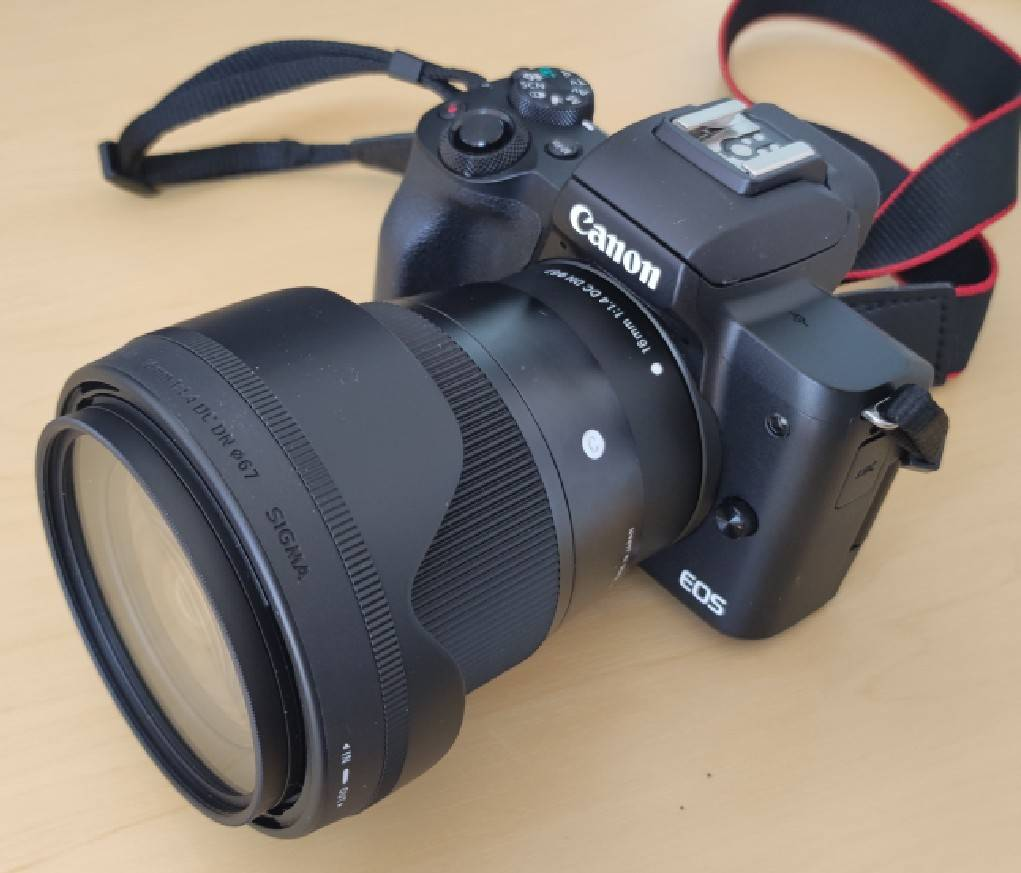
\includegraphics[width=8cm]{don.jpg}
		\caption{レンズをカメラに付けた感じ}
		\label{}
	\end{center}
\end{figure}
\section{試し撮り感想}
早速試し撮りをしに、晴れてる日の植物公園に行きました。どちらもシャッタースピード10秒、ISO 100で撮影しました。
\begin{figure}[H]
	\begin{center}
		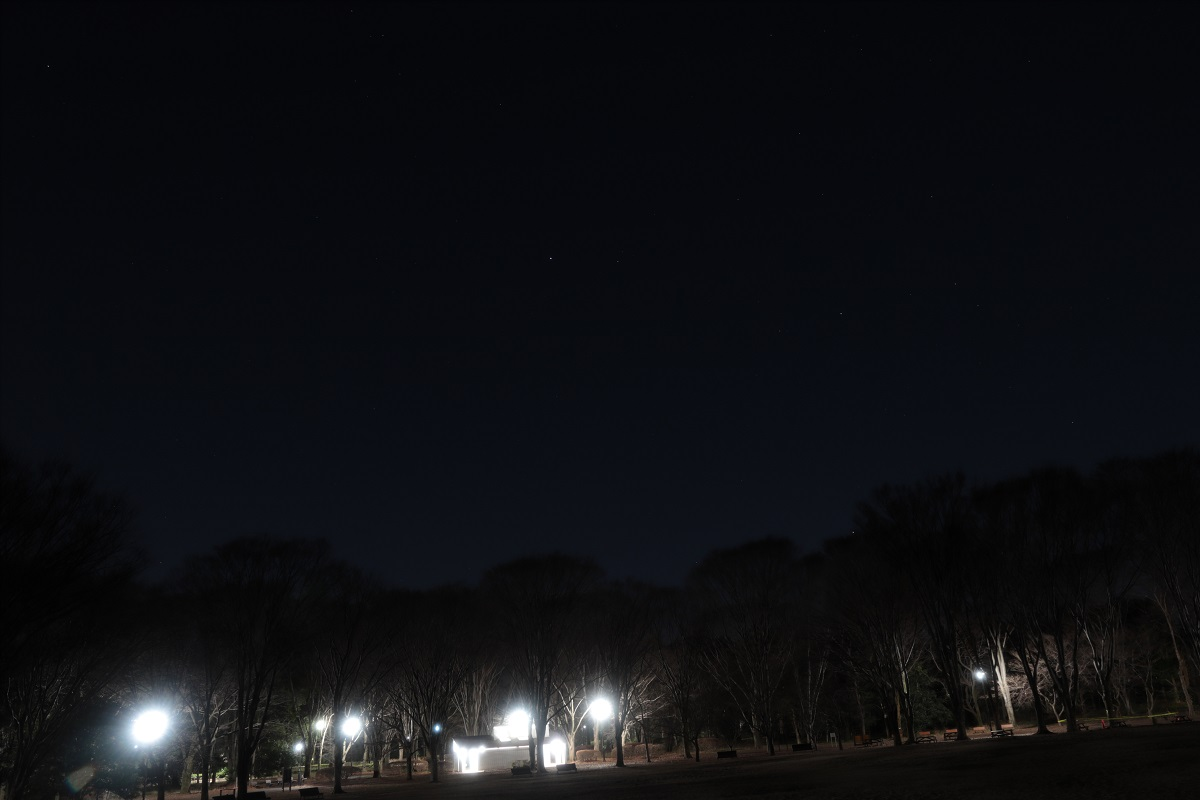
\includegraphics[width=12cm]{kurai.jpg}
		\caption{F3.5で撮影}
		\label{}
	\end{center}
\end{figure}
\begin{figure}[H]
	\begin{center}
		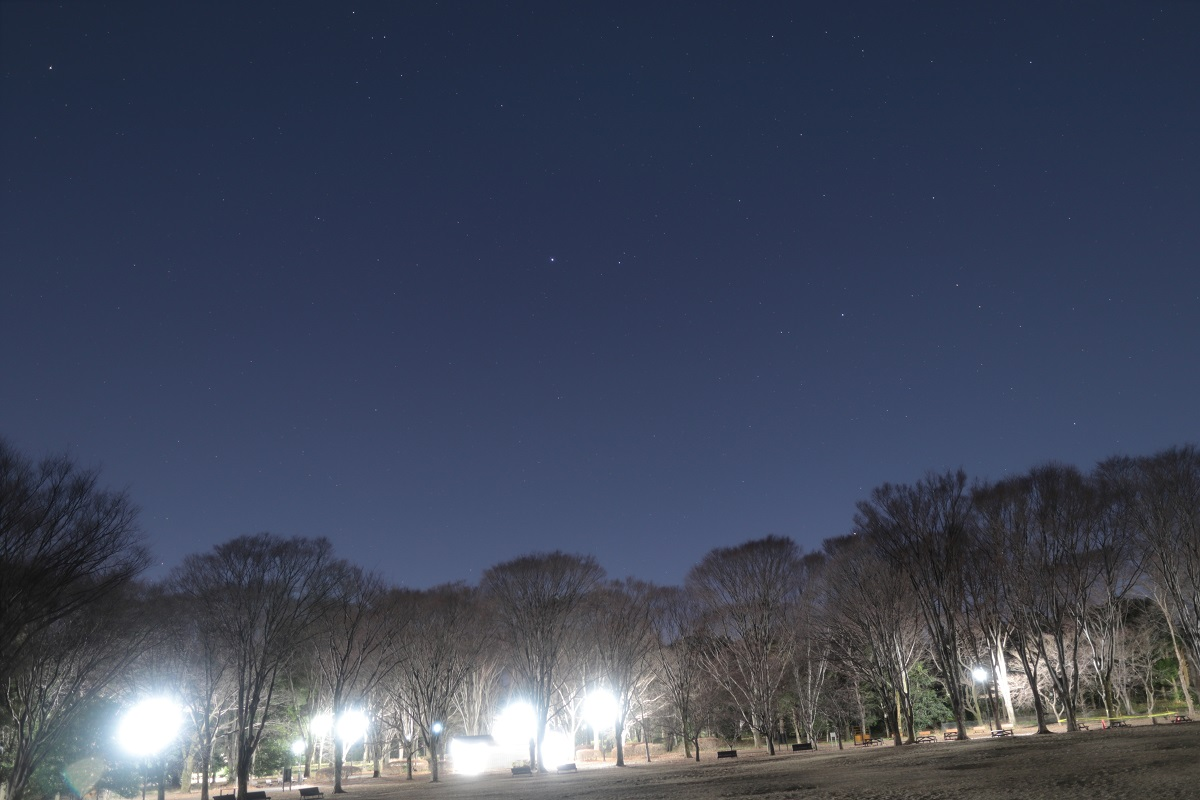
\includegraphics[width=12cm]{akarui.jpg}
		\caption{F1.4で撮影}
		\label{}
	\end{center}
\end{figure}
全然違いますね。明るいはすごい!F値は正義!\\
レンズ買ったのに合わせてソフトフィルター\footnote{定番のkenkoプロソフトンクリア}と光害カットフィルター\footnote{マルミのStarScape、光路差が出にくいらしいのでスターリーナイトでなくこちらを採用}も買ったのでついでにその比較画像も載せておきます。ソフトフィルターは光を滲ませるもので明るい星が目立つように写ります。光害カットフィルターは星空を撮る上で妨げとなる人工の光を抑えてくれるものです。いずれもシャッタースピード10秒、ISO 100、F1.6で撮影しました。
\begin{figure}[H]
	\begin{center}
		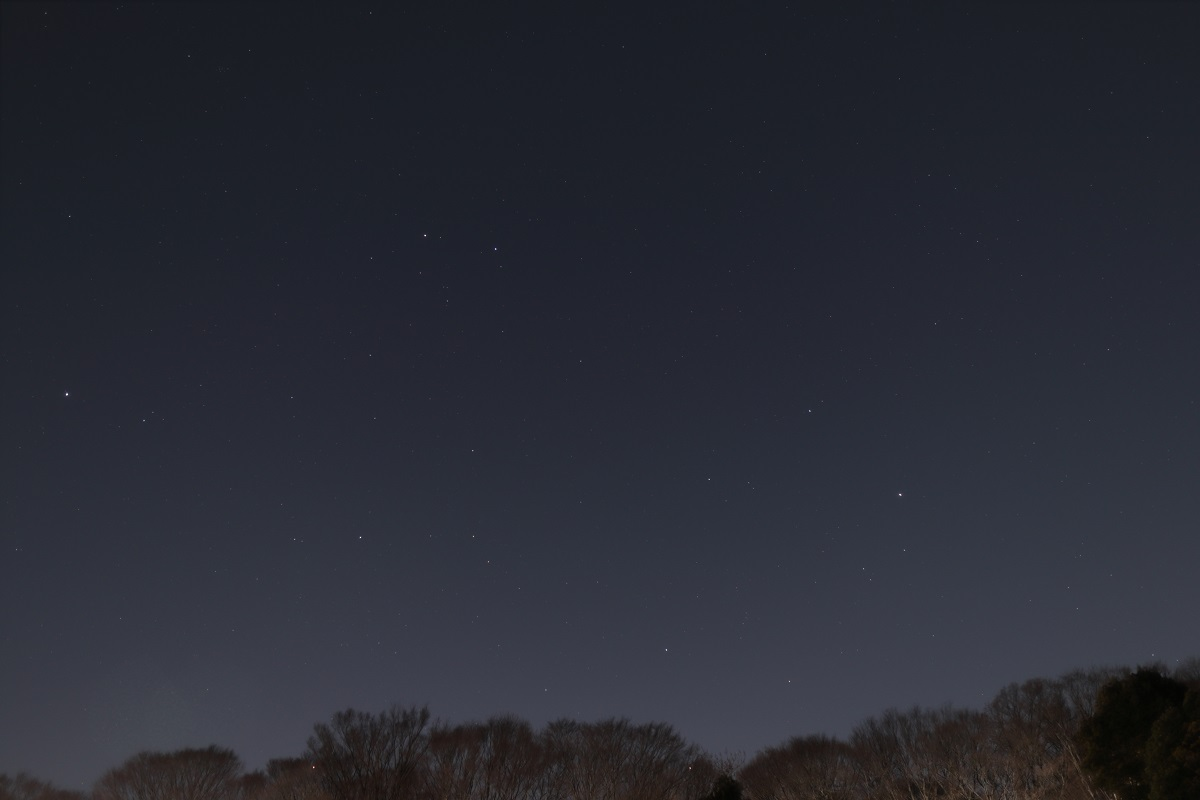
\includegraphics[width=14cm]{full.jpg}
		\caption{ソフトフィルターと光害カットフィルター装着}
		\label{}
	\end{center}
\end{figure}
\begin{figure}[H]
	\begin{center}
		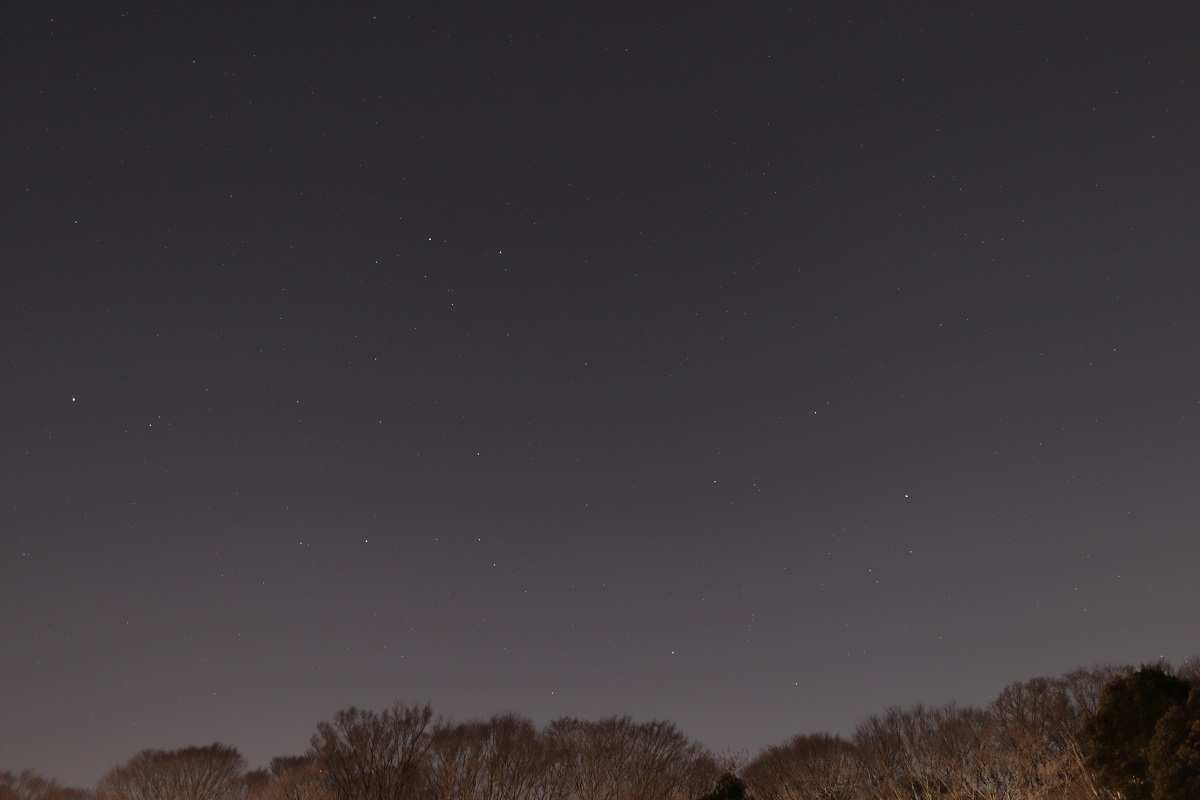
\includegraphics[width=14cm]{soft.jpg}
		\caption{ソフトフィルターのみ装着}
		\label{}
	\end{center}
\end{figure}
\begin{figure}[H]
	\begin{center}
		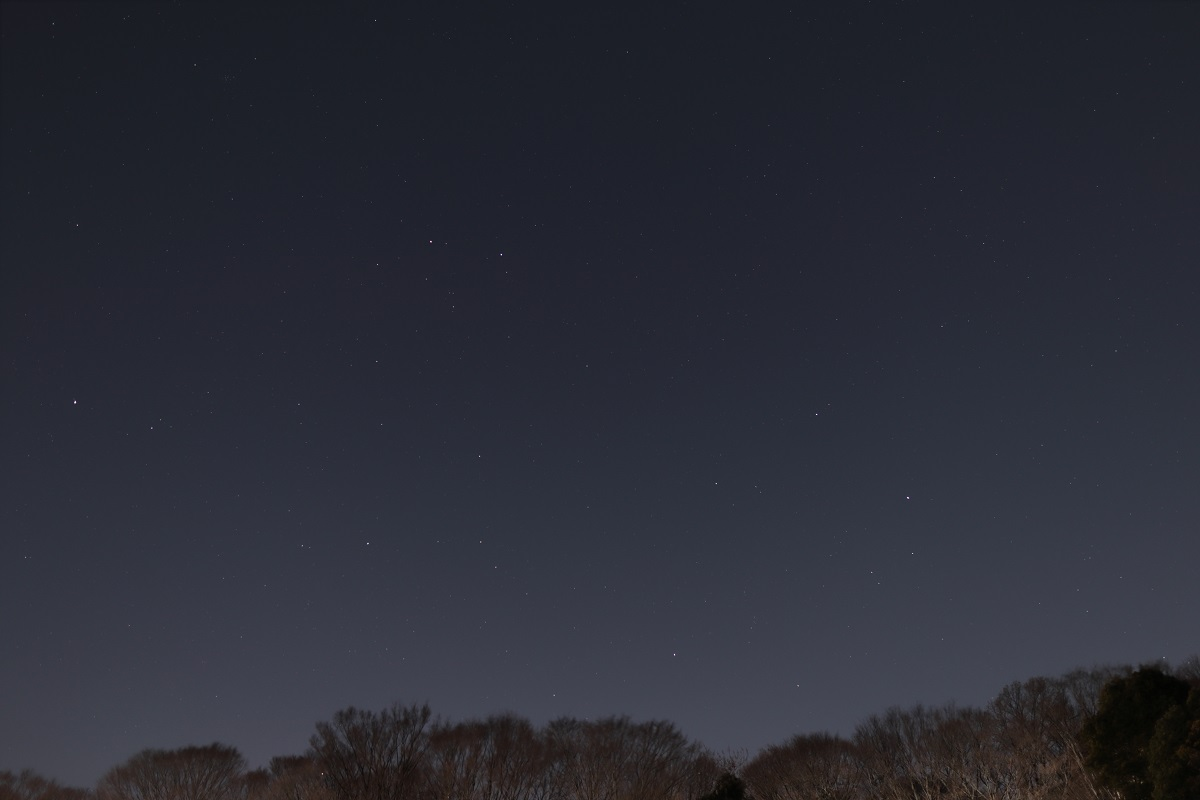
\includegraphics[width=14cm]{cut.jpg}
		\caption{光害カットフィルターのみ装着}
		\label{}
	\end{center}
\end{figure}
\begin{figure}[H]
	\begin{center}
		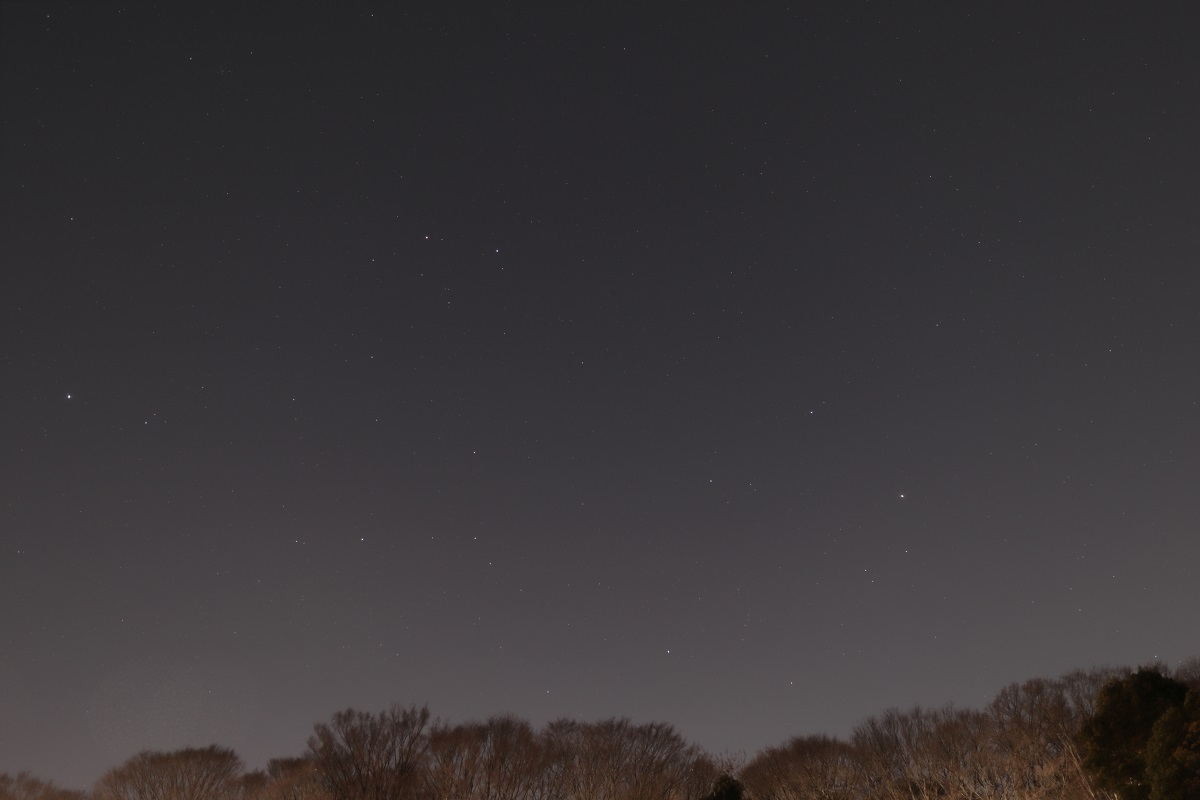
\includegraphics[width=14cm]{normal.jpg}
		\caption{素のレンズ}
		\label{}
	\end{center}
\end{figure}
なるべく大きな画像にしましたが、違いが分かりづらいですね。それでも光害カットフィルター装着では空の暗さが引き締まって良い印象です。ソフトフィルターは調布で撮る分にはあまり変わらないのですかね?ソフトフィルターの効果を実感する機会は合宿にお預けとなりそうです。\\
おまけで東京駅前kitteから夜景を撮影しました。シャッタースピード1/24秒で手持ちで撮りました。三脚なしで手持ちでもこれくらい撮れるなら満足ですよね。買った価値があります。
\begin{figure}[H]
	\begin{center}
		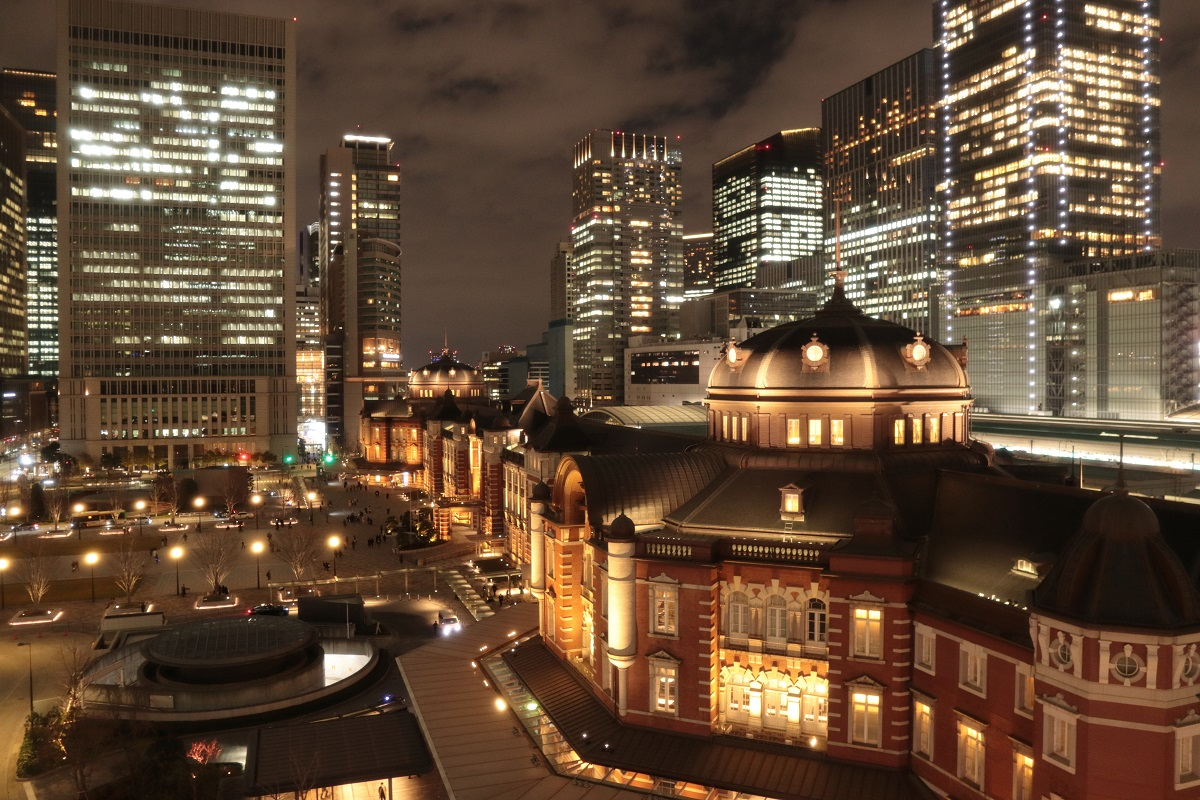
\includegraphics[width=14cm]{tokyo.jpg}
		\caption{夜景試し撮り}
		\label{}
	\end{center}
\end{figure}
\section{結論\footnote{あくまで個人の意見です}}
星空撮影界隈ではたまに機材よりもスキル\footnote{本当に大事なのは撮る環境}なんて言われることもありますが、結局良い機材があるに越したことはないんですよね。もちろん基本の撮影方法を知っていることはとても大事ですが、良いカメラ、良いレンズは良い!!光害カットフィルターも想像以上の効果が感じれたので持っていて損はないと言えます。最後に一言「みんなも明るいレンズを買おう!!」

\end{document}